\documentclass[12pt]{article}

\usepackage{xcolor} % For defining and using colors
\usepackage{amsmath} % For advanced math environments and equation formatting
\usepackage{amsfonts} % For additional math fonts and symbols
\usepackage{listings} % For displaying formatted source code
\usepackage{geometry} % For customizing page margins and layout
\usepackage{graphicx} % For inserting and scaling graphics/images
\usepackage[utf8]{inputenc} % For UTF-8 character encoding support

\geometry{a4paper, margin=1in}


% Define colors for code listings
\definecolor{codegreen}{rgb}{0, 0.6, 0}
\definecolor{codegray}{rgb}{0.5, 0.5, 0.5}
\definecolor{codepurple}{rgb}{0.58, 0, 0.82}
\definecolor{backcolour}{rgb}{0.95, 0.95, 0.92}


\lstset{
    backgroundcolor=\color{backcolour},
    commentstyle=\color{codegreen},
    keywordstyle=\color{magenta},
    numberstyle=\tiny\color{codegray},
    stringstyle=\color{codepurple},
    basicstyle=\ttfamily\footnotesize,
    breakatwhitespace=false,
    breaklines=true,
    captionpos=b,
    keepspaces=true,
    numbers=left,
    numbersep=5pt,
    showspaces=false,
    showstringspaces=false,
    showtabs=false,
    tabsize=2
}


\begin{document}


\begin{center}
    \textbf{\large ME 4511: Fluid Mechanics II} \\
    \vspace{0.5em}
    \textbf{Assignment 1} \\
    \vspace{0.5em}
    \textit{Abdullah al Azmi, 220011230}
    \vspace{1em}
\end{center}


\noindent \textbf{Q1} Here, the velocity field is:
\begin{align}
    u &= a(x^2-y^2) \\
    v &= -2axy
\end{align}


\begin{enumerate}

    \item[\textbf{(i)}] We assumed that the flow is \textbf{incompressible}, and we know that for a 2D incompressible, and steady flow, a stream function $\psi$ exists if it satisfies the continuity equation:
    
    \begin{equation*}
        \frac{\partial u}{\partial x} + \frac{\partial v}{\partial y} = 0
    \end{equation*}

    Now, calculating the partial derivatives:
    
    \begin{equation*}
        \frac{\partial u}{\partial x} = \frac {\partial}{\partial x}[a(x^2-y^2)] = 2ax
    \end{equation*}

    \begin{equation*}
        \frac{\partial v}{\partial y} = \frac{\partial}{\partial y}[-2axy] = -2ax
    \end{equation*}
    
    Substituting into the continuity equation:
    
    \begin{equation*}
        2ax + (-2ax) = 0
    \end{equation*}
    
    Since, the continuity equation is satisfied, a stream function does exist for this flow.

    \vspace{1em}
    
    \item[\textbf{(ii)}] Now, we obtain an expression for stream function $\psi$ and velocity potential $\phi$.

    \vspace{1em}

    Before that we have to verify whether a velocity potential exists for this 2D incompressible, and steady flow or not. A velocity potential $\phi$ exists if the flow is irrotational, which means that the vorticity $\omega$ must be zero:

    \begin{equation*}
        \omega = \frac{\partial v}{\partial x} - \frac{\partial u}{\partial y}
    \end{equation*}

    Calculating the partial derivatives:
    \begin{equation*}
        \frac{\partial v}{\partial x} = \frac{\partial}{\partial x}[-2axy] = -2ay
    \end{equation*}

    \begin{equation*}
        \frac{\partial u}{\partial y} = \frac{\partial}{\partial y}[a(x^2-y^2)] = -2ay
    \end{equation*}

    Substituting into the vorticity equation:

    \begin{equation*}
        \omega = -2ay - (-2ay) = 0
    \end{equation*}

    Since the vorticity is zero, the flow is irrotational, and thus a velocity potential $\phi$ exists for this flow.

    \vspace{1em}
    
    \textit{\textbf{a.} Stream Function ($\psi$):} By definition, we know that $u = \frac{\partial \psi}{\partial y}$ and $v = -\frac{\partial \psi}{\partial x}$
    
    \begin{equation*}
        \frac{\partial \psi}{\partial y} = a(x^2-y^2) \implies \psi = \int a(x^2-y^2)dy = ax^2y-\frac{ay^3}{3} + f(x)
    \end{equation*}

    To find $f(x)$, we use the other definition of stream function:
    \begin{equation*}
        -\frac{\partial \psi}{\partial x} = -\frac{\partial}{\partial x}\left(ax^2y-\frac{ay^3}{3} + f(x)\right) = -2axy + f'(x)
    \end{equation*}

    Setting this equal to $v$:
    
    \begin{equation*}
        -2axy + f'(x) = -2axy \implies f'(x) = 0 \implies f(x) = c
    \end{equation*}

    Therefore, the stream function is:

    \begin{equation*}
        \psi = a\left(x^2y - \frac{y^3}{3}\right) + c
    \end{equation*}

    \textit{\textbf{b.} Velocity Potential ($\phi$):} By definition, we also know that $u=\frac{\partial \phi}{\partial x}$ and $v=\frac{\partial \phi}{\partial y}$

    \begin{equation*}
        \frac{\partial \phi}{\partial x} = a(x^2-y^2) \implies \phi=\int a(x^2-y^2)dx = a\left(\frac{x^3}{3}-xy^2\right) + g(y)
    \end{equation*}

    To find $g(y)$, we use the other definition of velocity potential:

    \begin{equation*}
        \frac{\partial \phi}{\partial y} = \frac{\partial}{\partial y}\left(a\left(\frac{x^3}{3}-xy^2\right) + g(y)\right) = -2axy + g'(y)
    \end{equation*}

    Setting this equal to $v$:

    \begin{equation*}
        -2axy + g'(y) = -2axy \implies g'(y) = 0 \implies g(y) = c
    \end{equation*}

    Therefore, the velocity potential is:

    \begin{equation*}
        \phi = a\left(\frac{x^3}{3}-xy^2\right) + c
    \end{equation*}

    \vspace{1em}

    \item[\textbf{(iii)}] Plot of Stream Function for $C$ varying from -230 to 230 and $a=1$:
    
    \begin{figure}[ht]
        \centering
        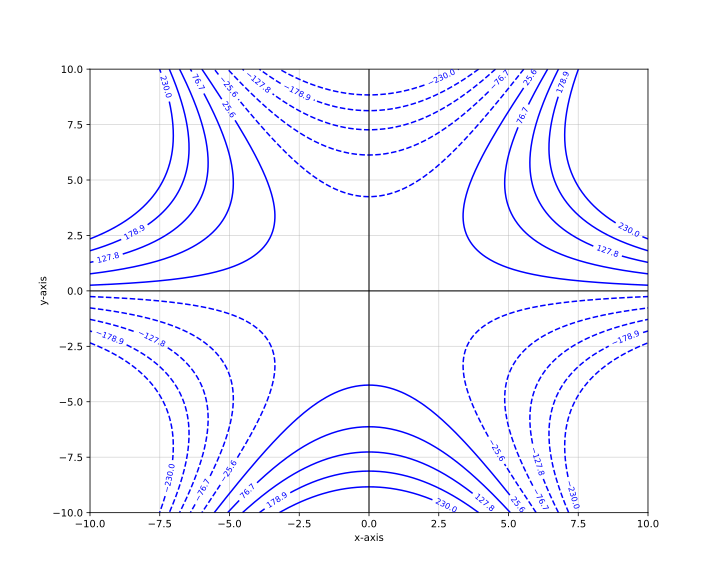
\includegraphics[width=1\textwidth]{stream_function_plot.png}
        \caption{\textit{Stream Function Contours for $C$ varying from -230 to 230}}
    \end{figure}
    
    \vspace{1em}
    
    \begin{lstlisting}[language=Python]

    import numpy as np
    import matplotlib.pyplot as plt

    a_val = 1  
    c_values = np.linspace(-230, 230, 10)

    x = np.linspace(-10, 10, 400)
    y = np.linspace(-10, 10, 400)
    
    X, Y = np.meshgrid(x, y)

    psi = a_val * (X**2 * Y - (Y**3)/3)
    
    c = plt.contour(X, Y, psi, levels=c_values, colors='blue')
    
    plt.figure(figsize=(10, 8))
    plt.clabel(c, inline=True, fontsize=8)
    plt.xlabel('x-axis')
    plt.ylabel('y-axis')
    plt.grid(True, alpha=0.5)
    plt.axhline(0, color='black', lw=1)
    plt.axvline(0, color='black', lw=1)
    plt.savefig('stream_function_plot.png', dpi=300)
    plt.show()

    \end{lstlisting}

\end{enumerate}

\vspace{1.5em}
\hrule
\vspace{1.5em}

\noindent \textbf{Q2}

\vspace{1.5em}
\hrule
\vspace{1.5em}

\noindent \textbf{Q3} Image of a fluid flow (water) taken using my own image acquisition system (mobile camera):

\begin{figure}[ht]
    \centering
    \includegraphics[width=1\textwidth]{laminar_flow_image_horizontal.jpg}
    \caption{\textit{Fluid Flow (Water) Image}}
\end{figure}

\begin{enumerate}

    \item [\textbf{(i)}] I have captured the image of flowing water from the tap to the basin. The way I have captured this image is by controlling the knob of the tap using hand to have a laminar flow of water. Then, I used my mobile camera to take the picture of the flowing water.
    \item [\textbf{(ii)}] Yeah, it is laminar flow. Because the water stream appears smooth and orderly without any visible turbulence or chaotic motion, which are characteristic features of laminar flow.
    \item [\textbf{(iii)}] The 
    \item [\textbf{(iv)}]
    \item [\textbf{(v)}] 

\end{enumerate}

\vspace{1.5em}
\hrule
\vspace{1.5em}

\end{document}